% ============================================================
%  TEMPLATE ARTICLE DE RECHERCHE
%  Compatible avec pdfLaTeX / XeLaTeX / LuaLaTeX
% ============================================================

\documentclass[10pt, a4paper, twocolumn]{article}

% -----------------------------------------------------------
% PACKAGES ESSENTIELS
% -----------------------------------------------------------
\usepackage[utf8]{inputenc}          % Encodage UTF-8
\usepackage[T1]{fontenc}             % Encodage des polices
\usepackage[french]{babel}           % Langue française
\usepackage{lmodern}                 % Police Latin Modern
 
% Mise en page
\usepackage[
  top=2cm, bottom=2.5cm,
  left=1.4cm,  right=1.4cm,
  columnsep=0.8cm
]{geometry}

% Typographie & apparence
\usepackage{microtype}               % Amélioration microtypographique
\usepackage{setspace}                % Espacement des lignes
\usepackage{parskip}                 % Espacement entre paragraphes
\usepackage{titlesec}                % Personnalisation des titres
\usepackage{abstract}                % Personnalisation du résumé
\usepackage{fancyhdr}                % En-têtes et pieds de page

% Mathématiques
\usepackage{amsmath, amssymb, amsthm}
\usepackage{mathtools}

% Figures & tableaux
\usepackage{graphicx}                % Inclusion d'images
\usepackage{float}                   % Placement précis des figures
\usepackage{booktabs}                % Tableaux professionnels
\usepackage{caption}                 % Légendes personnalisées
\usepackage{subcaption}              % Sous-figures
\usepackage{listings}				 % Intégration de ligne de code


\lstset{
    basicstyle=\ttfamily\footnotesize,
    breaklines=true,
    breakatwhitespace=true,
    columns=flexible
}

% Couleurs
\usepackage[dvipsnames]{xcolor}
\definecolor{accentcolor}{RGB}{0, 75, 135}  % Bleu académique

% Hyperliens & références
\usepackage[
  colorlinks=true,
  linkcolor=accentcolor,
  citecolor=accentcolor,
  urlcolor=accentcolor,
  pdftitle={Titre de l'article},
  pdfauthor={Auteur(s)},
]{hyperref}
\usepackage[
  backend=biber,
  style=numeric,
  sorting=none
]{biblatex}                          % Bibliographie (nécessite biber)
\addbibresource{references.bib}      % Fichier .bib

% Divers
\usepackage{lipsum}                  % Texte de remplacement (à supprimer)
\usepackage{csquotes}                % Guillemets adaptés à la langue
\usepackage{enumitem}                % Listes personnalisées

% -----------------------------------------------------------
% THÉORÈMES & DÉFINITIONS
% -----------------------------------------------------------
\newtheorem{theorem}{Théorème}[section]
\newtheorem{lemma}[theorem]{Lemme}
\newtheorem{corollary}[theorem]{Corollaire}
\newtheorem{proposition}[theorem]{Proposition}
\theoremstyle{definition}
\newtheorem{definition}{Définition}[section]
\theoremstyle{remark}
\newtheorem{remark}{Remarque}[section]

% -----------------------------------------------------------
% STYLE DES SECTIONS
% -----------------------------------------------------------
\titleformat{\section}
  {\large\bfseries\color{accentcolor}}
  {\thesection.}{0.5em}{}[\titlerule]

\titleformat{\subsection}
  {\normalsize\bfseries}
  {\thesubsection.}{0.5em}{}

\titleformat{\subsubsection}
  {\normalsize\itshape}
  {\thesubsubsection.}{0.5em}{}

% -----------------------------------------------------------
% EN-TÊTES & PIEDS DE PAGE
% -----------------------------------------------------------
\pagestyle{fancy}
\fancyhf{}
\fancyhead[L]{\small\textit{TOP}}
\fancyhead[R]{\small\textit{Bauer Théo - Nolwen Dolléans}}
\fancyfoot[C]{\thepage}
\renewcommand{\headrulewidth}{0.4pt}

% -----------------------------------------------------------
% STYLE DU RÉSUMÉ
% -----------------------------------------------------------
\renewcommand{\abstractnamefont}{\bfseries\color{accentcolor}}
\setlength{\absleftindent}{0pt}
\setlength{\absrightindent}{0pt}

% -----------------------------------------------------------
% MÉTADONNÉES DE L'ARTICLE
% -----------------------------------------------------------
\title{%
  \vspace{-1.5cm}
  \rule{\linewidth}{0.5pt} \\[0.5em]
  {\LARGE \textbf{Optimization of an hybrid parallel D2Q9 lattice Boltzmann solver for Kármán vortex street}} \\[0.2em]
  {\large Technique d'Optimisation de la Parallélisation}
}

\author{%
  \textbf{Bauer Théo} \quad
  \textbf{Nolwen Dolléans} \\[0.4em]
  \small M1 - CHPS \\
}

\date{%
  \small Soumis le : \today
}

% ============================================================
%  DÉBUT DU DOCUMENT
% ============================================================
\begin{document}

% ------- Page de titre ----------------------------------------
\twocolumn[
  \maketitle
  % \vspace{-0.5em}
  % \rule{\linewidth}{1.5pt}
  % \vspace{0.5em}

  % ------- Résumé (sur toute la largeur) ----------------------
  % \begin{onecolabstract}
  % \bigskip
  %   % \input{resume.tex}
    
  % \end{onecolabstract}

  % \vspace{1em}
  \rule{\linewidth}{1.5pt}
  \vspace{1em}
]

% -----------------------------------------------------------
% 1. INTRODUCTION
% -----------------------------------------------------------
\section{Introduction}

Ceci est un projet d'optimisation d'un programme parallèle de simulation de mécanique des fluides en language C++ dans un contexte d'études en Calcul Haute Performance.

L'objectif principal est d'analyser les performances du code existant, d'identifier les principaux goulets d'étranglement, puis de proposer et mettre en oeuvre des optimisations visant à améliorer son efficacité à l'aide principalement d'outils de profiling afin de rendre le programme le plus scalable possible.

La parallélisation est réalisé grâce aux librairies MPI et OpenMP, visant à profiter du modèle physique pour adapter la simulation sur des architectures HPC.


%-----------------------------------------------------------
% 2. Analyse du code initial
% -----------------------------------------------------------
\section{Analyse du code initial}

Le code originale se structure comme suit:
\begin{enumerate}
	\item Une phase d'initialisation.
	\item Envoie des cellules fantômes.
	\item Calcul de la vitesse des particules fluides et de la densité de ce dernier en tous points.
	\item Actualisation de la position du fluide.
	\item Envoie des cellules fantômes.
	\item ...
\end{enumerate}
De ce fait, nous pouvons extraire 2 grands axes d'optimisation: S'assurer que l'envoie de message est optimal ainsi que celui du calcul. 

% -----------------------------------------------------------
% 3. Optimisations apportées
% -----------------------------------------------------------
\section{Optimisations apportées}

Nous utiliserons plusieurs outils de profiling pour déceler les points chauds du programme:
\begin{itemize}
	\item[$\bullet$] \textit{Instruments.app}: Flame Graph, nombre d'instructions et de cycles CPU, IPC (Instructions per cycles) moyens
	\item[$\bullet$] \textit{perf}: Mesure des IPC, cache-misses, cache-references par fonction
	\item[$\bullet$] \textit{gdb}: Débuggage, évaluation de l'évolution des variables et repérage de crash.
\end{itemize}
	
Tout graphique et résultats d'outils de profiling seront mis en annexes.

\subsection{Première approche}
Afin de commencer à chercher les premières optimisations, nous avons tracer un Flame graph du programme (cf \hyperref[fig:flamegraph1]{Annexe A}). Nous pouvons ainsi nous rendre compte que les communications MPI pour un maillage en halo sont le point chaud majeur, et ralentissent significativement le programme. C'est donc la première chose sur laquelle nous allons nous concentrer.

\subsection{Optimisation des communications MPI}
La première de ces optimisations est le fait de retirer le 2e envoi de maille fantôme vers la gauche, puisqu'il n'est pas nécessaire de le faire 2 fois.

 Nous constatons que les performances sont réduites à cause de 3 fonctions MPI: \textit{MPI\_Barrier}, \textit{MPI\_Send} et \textit{MPI\_Recv} dans la fonction \textit{lbm\_comm\_halo\_exchange} (cf \hyperref[section:AnnexeB]{Annexe B}). Nous allons donc repenser comment les mailles fantômes sont envoyées.\\
 Les \textit{MPI\_Barrier} sont un problème majeur dans cette fonction. En effet, il est inutile de mettre des MPI\_Barrier ici, puisque le buffer envoyé est différent pour chacune des fonctions d'envoi et les communications étant bloquante, la synchronisation est déjà incluse.\\
 Comme dit précédemment, les buffers envoyés par communication sont différents (cf. \hyperref[fig:exchange]{Figure 1}).
 \begin{figure}[H]
  \centering
  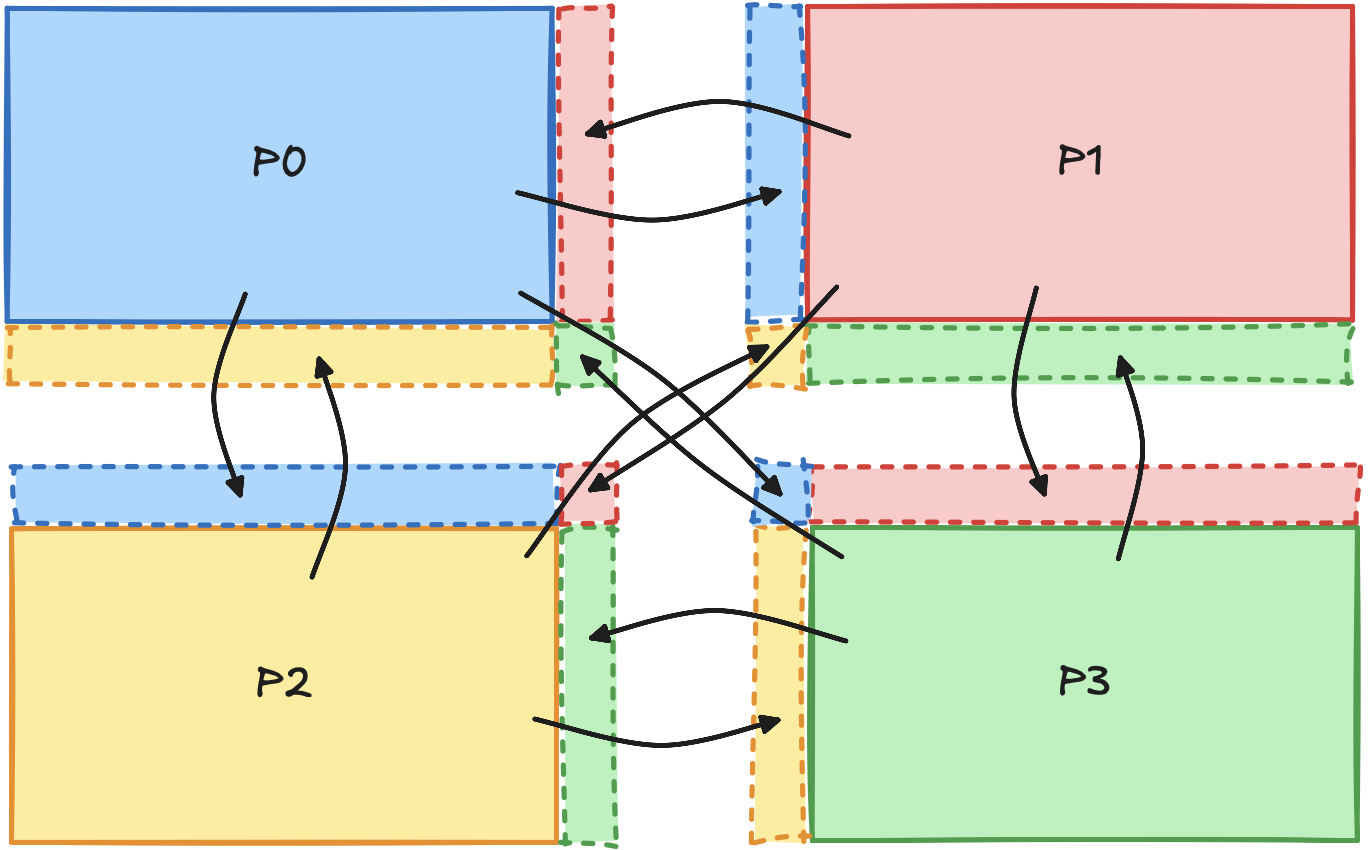
\includegraphics[scale=0.35]{graphs/lbm-comm_scheme.png}
  \caption{Halo exchange communication scheme for 4 MPI processes}
  \label{fig:exchange}
\end{figure}

Ainsi, nous pouvons utiliser des communications non-bloquantes sur chacune des fonctions d'envoi de mailles à l'aide de \textit{MPI\_Isend} et \textit{MPI\_Irecv}, avec un \textit{MPI\_Waitall} à la place de la série de \textit{MPI\_Barrier}, pour s'assurer que le programme calcul sur une zone qui n'a pas encore été complètement reçue puis avons ajouter un tag unique en fonction du rang et de la direction de la communication afin que les communications soient déterministes. Ceci sera notre première optimisation.

Nous avons également remarquer d'autres \textit{MPI\_Barrier} au sein même de la boucle de calcul entre chaque étape, forçant les processus MPI à se synchroniser après le calcul des collisions, de l'échange de mailles fantômes et du calcul de la propagation. Or, cela est sans justification car les processus ont besoin d'être synchronisés uniquement lors de l'envoi de message, pour éviter d'entamer le calcul sur des buffers qui ne sont pas encore pleinement envoyés. Nous pouvons ainsi supprimer l'entièreté des \textit{MPI\_Barrier}.\\

A l'heure actuelle, la division des processus MPI se fait de la manière suivante:
\begin{enumerate}
	\item nombre de processus en x: par le PGCD de la longueur par le nombre de processus MPI
	\item nombre de processus en y: $\tfrac{Nombre\ de\ processus}{nombre\ de\ processus\ en\ x}$
\end{enumerate}

 \vspace{0.1cm}
 Cette répartition naïve fonctionne, mais réparti les processus en chaîne et non en halo. En effet, PGCD de comm\_size et width vaut comm\_size dès que comm\_size divise width, on se retrouve donc avec une répartition de (comm\_size x 1). De plus, cette méthode ne prend pas en compte la taille de la conduite: le PGCD sera toujours égal au nombre de processus en x, même si la largeur est plus grande que la longueur.\\
 Une modification que l'on peut apporter est de trouver un $nb_{x}$ et un $nb_{y}$ tels que:

 $$\left\{{\frac{width}{nb_x}=\tfrac{height}{nb_y}\atop nb_x*nb_y=comm\_size}\right.$$
 $$\implies\left\{{nb_x=\sqrt{comm\_size\tfrac{width}{height}}\atop nb_y=comm\_size / nb_x}\right.$$
\\

Cependant, comme $nb_x$ et $nb_y$ sont des entiers, afin de limiter des erreurs suite à des conversions de flottants, nous avons choisi de faire cette algorithme:
on détermine la paire $\left(i\leq comm\_size, j= comm\_size/i\right)$ minimisant la fonction suivante $\left|j - \sqrt{comm\_size \times width / height}\right|$.\\
Ceci permettra de trouver le meilleur couple qui suit la longueur et la largeur: plus la largeur est grande, plus il y aura de nombre de processus en y, et inversement. Cela nous permettra d'avoir une topologie en halo et non en chaîne dans la majorité des cas.\\

Nous en profiterons également pour revisiter la manière dont les cellules fantômes sont envoyés horizontalement. En effet, pour ces communications, les processus envoient une colonne de cellules qui ne peuvent se faire un 1 seul message, contrairement aux envois verticaux, les colonnes n'étant pas contiguës en mémoire en C++. Heureusement, il est possible de le faire en 1 message par le biais de vecteur MPI\footnote{Source: https://www.to.infn.it/~mignone/MPI/lecture4.pdf}. Cela nous permet de faire un Datatype MPI permettant de faire un vecteur composé de \textit{mesh->height - 2} quantité de \textit{DIRECTIONS} doubles, avec un stride de \textit{mesh->width * DIRECTIONS}. Ainsi, il suffit d'envoyer 1 vecteur de ce type par message pour envoyer une colonne en entier.

\subsection{Implémentation OpenMP}

La fonction \textit{main} comporte une boucle for sur le nombre d'itérations à réaliser pour la simulation (dans notre cas, 20,000 itérations) qui fait appel à plusieurs fonctions qui sont parallélisables dans un contexte multi-thread. C'est pourquoi nous avons englober cette partie dans une région parallèle OpenMP, puis nous avons réparti la charge de travail des threads à l'intérieur de ces fonctions parallélisables. Pour celles qui ne le sont pas nous avons rajoutons un "single".

Parmis les fonctions parallélisables nous retrouvons \textit{special\_cells}, \textit{collision} et \textit{propagation} qui font appel des boucles for sur la height et la width. Puisque par la division des taches entre processus MPI, nous avons réparti la height entre processus, alors nous allons répartir les taches sur la width entre les threads. Nous posons pour ces trois fonctions une parallélisation de la seconde boucle for sous un ordonnancement dynamique (déterminé expérimentalement avec plusieurs tailles de blocs comme étant la meilleure solution sur des coeurs à 2 coeurs logiques, répartissant MPI sur les coeurs physiques et OpenMP sur les hyperthreads).

Notons que nous devons laisser la barrière implicite à la fin de la boucle parallélisée afin d'assurer que les résultats restent justes.

\subsection{Optimisation mémoire}

Nous avons réaliser une première mesure du ratio $\dfrac{cache-misses}{cache-references}$ de chacune des fonctions du programme grace à perf, deux fonctions montraient un fort pourcentage de cache-misses, montrant une mauvaise utilisation de la mémoire. Ces fonctions sont (cf. \hyperref[fig:perf-naive]{Annexe D}):
\begin{itemize}
	\item[$\bullet$] \textit{collision} qui appelle \textit{compute\_cell\_collision} et a 47.29\% de cache-miss rate
	\item[$\bullet$] \textit{propagation} a 26.70\% de cache-miss rate 
\end{itemize}
En analysant ces fonctions, nous voyons que nous gérons les tableaux Mesh::cell de taille $width\times height\times DIRECTIONS = 802\times (\dfrac{162}{\text{mpi\_size}})\times 9$. Leur type est des doubles, ce qui rend ces tableaux grands, il faut donc s'assurer de profiter de la localité temporelle des données afin d'éviter d'évincer la mémoire à cause d'autres variables ou calculs trop rapidement. En regardant la fonction \textit{Mesh\_get\_cell} qui défini le "first-touch" sur ces tableaux, nous voyons que l'ordonnancement des tableaux est [height][width][DIRECTIONS], c'est pourquoi nous avons commencer par structurer l'ensemble des accès aux données dans tout le code comme un triple boucle for dans ce sens là. C'est-à-dire interchanger les boucles en width et height dans l'ensemble des fonctions ayant cette boucle for.

Commençons par la fonction \textit{collision} : 

Nous avons décider d'éviter de réaliser des appels de fonctions. En effet, \textit{get\_cell\_velocity} et \textit{compute\_equilibrium\_profile} ne sont pas inline car elles sont également appelées dans "initialization.cpp" et sont facilement adaptées pour une implémentation directe. Cependant, nous définissons \textit{compute\_cell\_collision} comme étant inline. Nous initialisons la plupart des variables en dehors de la triple boucle for afin de réutiliser leurs localité mémoire, puis nous allégeons les calculs en terme d'opérations, par exemple de "f\_eq".

Ensuite pour la fonction \textit{propagation} :

Avant d'optimiser cette fonction, dans la version de base, la comparaison des résulats avec la référence était fausse, et avions besoin de corriger le fait que ce soti 

Deux principaux problèmes à optimiser ont été recontrés ici : le premier est en relation avec les types des variables. Nous avons i,j,k des size\_t; ii,jj des ssize\_t; direction\_matrix[k][] des doubles; mesh\_out->width, mesh\_out->height des uint32\_t; \textit{Mesh\_get\_cell} qui prend en argument des int. Les parenthèses sur la lignes ssize\_t ii = (i + direction\_matrix[k][0]); assure un premier cast de i en double pour une somme en double, puis un cast en ssize\_t pour obtenir le résultat. Tout comme la fonction précédente, nous avons initiliaser au début de l'appel de la fonction les différentes variables et avons tout définis en tant que int pour éviter le plus de conversions possibles.

Le deuxième problème est la condition dans la triple boucle for, en analysant l'utilisation de cette fonction, nous voyons que c'est l'avant-dernière fonction de la boucle for dans \textit{main} avant \textit{save\_frame\_all\_domain}. Or cette dernière n'opère pas sur les cellules fantômes, nous retirons donc des opérations sur les boucles en j et i; cela vient également éviter d'avoir des valeurs de j et i très grandes lorsque i=0 et direction\_matrix[k][0]=-1.0 par exemple. 

Suite à ces optimisations, nous avons réévaluer dans les mêmes conditions les mesures de perf pour le cache-miss ratio (cf. \hyperref[fig:perf-naive]{Annexe D}):
\begin{itemize}
	\item[$\bullet$] \textit{collision} a 5.00\% de cache-miss rate
	\item[$\bullet$] \textit{propagation} a 5.72\% de cache-miss rate 
\end{itemize}

Nous notons donc une grande différence, non seulement dans le ratio, mais également dans le nombre de références éffectuées : 70 milliards contre 37 milliards, montrant bien une meilleure localité temporelle de la mémoire sur les parties les plus importantes du programme.

\subsection{Autres optimisations}

\subsubsection{MPI\_Syncall}

Une optimisation notable réalisée est en relation avec la fonction \textit{MPI\_Syncall} appelée à la fin de la fonction établissant les communications. Or cette fonction ne fait pas partie de la librairie MPI.

Dans le code, tout ce qui est en relation avec MPI\_Syncall se trouve ici :

\begin{minipage}{0.48\textwidth}
\begin{lstlisting}[language=C]
MPI_Syncall(MPI_COMM_WORLD);

static MPI_Syncfunc_t* MPI_Syncall = PMPI_Syncall_cb;

static int PMPI_Syncall_cb(MPI_Comm comm) {
  static int (*__builtin_fence_ps)() = rt_tpl_sync(comm, __builtin_fence_ps, MPI_HINT_VTBL);
  return __builtin_fence_ps();
}

#define rt_tpl_sync(comm,fence,sym) catof(resolve,_tpl,_sync)<decltype(fence)>(sym)

#define catof(a,b,c) a##b##c

#define MPI_HINT_VTBL "5f5f6275696c74696e5f73796e635f66656e63655f"
\end{lstlisting}
\end{minipage}

Nous essayons donc de retracer ce que cela veut dire, premierement, nous interpretons que :

\begin{minipage}{0.48\textwidth}
\begin{lstlisting}[language=C]
PMPI_Syncall_cb(MPI_COMM_WORLD) {
    __builtin_fence -> pointeur de fonction (?) qui devrait renvoyer un int
    return __builtin_fence; -> on appel la fonction
}
\end{lstlisting}
\end{minipage}

ce qui veut dire

\begin{minipage}{0.48\textwidth}
\begin{lstlisting}[language=C]
return catof(resolve,_tpl,_sync)
    <__builtin_fence_ps>(MPI_HINT_VTBL)
\end{lstlisting}
\end{minipage}

Puisque \_\_builtin\_fence\_ps est utilisé comme un type dans les <>, nous extrayons que c'est un int(*)(), nous avons alors :

\begin{minipage}{0.48\textwidth}
\begin{lstlisting}[language=C]
return resolve##_tpl##_sync<int(*)()>(
    "5f5f6275696c74696e"
    "5f73796e635f66656e"
    "63655f");
\end{lstlisting}
\end{minipage}

les hashtag servent a concaténer les arguments, donc :

\begin{minipage}{0.28\textwidth}
\begin{lstlisting}[language=C]
return resolve_tpl_sync<int(*)()>(
    "5f5f6275696c74696e"
    "5f73796e635f66656e"
    "63655f"
);
\end{lstlisting}
\end{minipage}

on retrouve la fonction resolve\_tpl\_sync dans le fichier build/include/lbm/tpl\_loader.hpp :

\begin{minipage}{0.48\textwidth}
\begin{lstlisting}[language=C]
template <typename F>
F resolve_tpl_sync(const std::string& tbl_addr) {
 void* sym = dlsym(RTLD_DEFAULT,hex_decode(tbl_addr).data());
 return reinterpret_cast<F>(sym);
}
\end{lstlisting}
\end{minipage}

avec :

\begin{minipage}{0.48\textwidth}
\begin{lstlisting}[language=C]
extern void *dlsym (void *__restrict __handle,
		    const char *__restrict __name) __THROW __nonnull ((2));

#define RTLD_DEFAULT	((void *) 0)
\end{lstlisting}
\end{minipage}

en remplaçant les arguments

\begin{minipage}{0.48\textwidth}
\begin{lstlisting}[language=C]
dlsym(RTLD_DEFAULT, hex_decode(
    "5f5f6275696c74696e"
    "5f73796e635f66656e"
    "63655f"
).data());
\end{lstlisting}
\end{minipage}

En apprenant par coeur les hex codes, il est trivial que 
5f5f6275696c74696e5f73796e635f66656e63655f = \_\_builtin\_sync\_fence\_
Donc :
dlsym(((void *) 0), "\_\_builtin\_sync\_fence\_");

Il parait que cette fonction retourne l'adresse d'un symbole de nom "\_\_builtin\_sync\_fence\_" dans toutes les librairies SHARED. Cela comprend en particulier top.lbm-lib, MPI ou OpenMP.

Nous appliquons ensuite reinterpret\_cast<int(*)()>(sym) ce qui rend cette adresse une fonction pointée que nous pouvons appeler, car nous faisons return de ce pointeur.

La fonction de nom "\_\_builtin\_sync\_fence\_" se trouve dans build/include/lbm/tpl.hpp et est définie comme un code en assembleur qui implique une veille de une seconde, sans raison particuliere.

Pour la retirer, puisque nous avons vu le contenu des deux fichiers "tpl\_loader.hpp" et "tpl.hpp" alors nous allons effacer la ligne 

\begin{minipage}{0.48\textwidth}
\begin{lstlisting}[language=C]
FILES ${CMAKE_BINARY_DIR}/include/lbm/tpl.hpp ${CMAKE_BINARY_DIR}/include/lbm/tpl_loader.hpp
\end{lstlisting}
\end{minipage}

du CMakeFile dans src/lbm, et effacer également toutes les lignes en relation avec MPI\_Syncall.

\subsubsection{Autres}

Nous avons retirer la fonction \textit{init\_cond\_velocity\_0\_density\_1} qui n'est pas utilisée.

En termes de linking : nous avons limiter les includes en fonction des dépendances des fichiers, et nous sommes assurer de ne pas inclure plusieurs fois les mêmes fichiers, par exemple inclure une fois dans un .hpp puis le même fichier dans le .cpp associé.

Les boucles for sur DIMENSIONS ont été déroulées car DIMENSIONS=2.







% -----------------------------------------------------------
% 4. MÉTHODOLOGIE 
% -----------------------------------------------------------
\section{Expériences}
\subsection{Protocole expérimental}

\lipsum[9]

\subsubsection{Jeux de données}

\lipsum[10]

\subsubsection{Hyperparamètres}

Les hyperparamètres utilisés sont récapitulés dans la Table~\ref{tab:hyperparams}.

\begin{table}[H]
  \centering
  \caption{Hyperparamètres de la configuration expérimentale.}
  \label{tab:hyperparams}
  \begin{tabular}{lcc}
    \toprule
    \textbf{Paramètre} & \textbf{Valeur} & \textbf{Plage testée} \\
    \midrule
    Taux d'apprentissage & $10^{-3}$ & $[10^{-4}, 10^{-2}]$ \\
    Taille du lot & 64         & $\{32, 64, 128\}$ \\
    Époques          & 100        & — \\
    Régularisation $\lambda$ & $10^{-4}$ & $[10^{-5}, 10^{-3}]$ \\
    \bottomrule
  \end{tabular}
\end{table}

\subsection{Résultats}

\lipsum[11]

% Exemple de tableau de résultats comparatifs
\begin{table}[H]
  \centering
  \caption{Comparaison des performances (\%) sur le jeu de test.}
  \label{tab:resultats}
  \begin{tabular}{lccc}
    \toprule
    \textbf{Méthode} & \textbf{Précision} & \textbf{Rappel} & \textbf{F1} \\
    \midrule
    Méthode A \cite{exemple2024} & 82.3 & 79.1 & 80.7 \\
    Méthode B & 85.6 & 83.2 & 84.4 \\
    \textbf{Notre approche} & \textbf{89.1} & \textbf{87.5} & \textbf{88.3} \\
    \bottomrule
  \end{tabular}
\end{table}

\subsection{Analyse et discussion}

\lipsum[12]

\begin{remark}
  Notons que les résultats présentés dans la Table~\ref{tab:resultats} ont été obtenus avec une validation croisée à 5 plis afin de garantir la robustesse statistique.
\end{remark}

% 

% -----------------------------------------------------------
% 5. RÉSULTATS
% -----------------------------------------------------------
\section{Résultats}

Voici un tableau récapitulatif des optimisations et leurs impacts sur le Mlups (cf \hyperref[tab:results_halo]{Table 2}), la valeur Mlups mesurée pour la version initale est $Mlups=125\pm3$:

\begin{table}[H]
  \centering
  \caption{Optimisation de la communication dans l'halo}
  \label{tab:results_halo}
  \begin{tabular}{lcc}
    \toprule
    \textbf{Optimisation} & \textbf{Mlups} & $\delta_{Mlups}$ \\
    \midrule
     Comm. non-bloquantes  & $1575$ & $\pm 20$\\
     Sup. \textit{MPI\_Barrier} main  & $2363$ & $\pm 20$\\
     Halo + 1 message / colonne  & $2503$ & $\pm 30$\\
    \bottomrule
  \end{tabular}
\end{table}

\begin{table}[H]
  \centering
  \caption{Optimisation memoire}
  \label{tab:results_memory}
  \begin{tabular}{lcc}
    \toprule
    \textbf{Optimisation} & \textbf{Mlups} & $\delta_{Mlups}$ \\
    \midrule
     Optimisation memoire  & $2830$ & $\pm 30$\\
    \bottomrule
  \end{tabular}
\end{table}


Discussions:\\
Nous remarquons que les améliorations faites sur les communications ont des conséquences plus importantes que l'amélioration sur la gestion de la mémoire.\\

% -----------------------------------------------------------
% 6. CONCLUSION
% -----------------------------------------------------------
\section{Conclusion}
Au long de l'analyse de ce programme, nous avons été capables de repérer divers types de problèmes optimisables. Que ce soit en lien avec le modèle de parallélisation, avec des phénomènes informatiques ou encore des observations directes de mesures de performances. Ces problèmes nous ont mener par la suite à une inspection fine du code et de compréhension du phénomène étudié.

Le résultat obtenu à ce jour est satisfaisant, la différence lors des comparaisons suite à chaque optimisations est notable et nous avons étudier une partie importante de l'ensemble du code.

Parmis les optimisations supplémentaires qui seraient réalisables nous comptons principalement la vectorisation. Les fonctions \textit{collision} et \textit{propagation} sont complètement vectorisables (après optimisation) mais nécessiteraient une approche différente de l'ordonnancement de la mémoire des tableaux des cellules, en particulier d'avoir la width contigüe en mémoire.

Finalement ce projet à été enrichissant et nous a obligé à appliquer concrètement diverses connaissances apprises au cours de cette année d'étude.

% -----------------------------------------------------------
% BIBLIOGRAPHIE
% -----------------------------------------------------------
\printbibliography[title={Références}]

% -----------------------------------------------------------
% APPENDICES (optionnel)
% -----------------------------------------------------------

\onecolumn 
\newpage

\begin{center}
  {\large\bfseries\color{accentcolor} Annexes}
\end{center}
\vspace{0.5em}

\appendix

\section{Flame Graph initial: Instruments.app}

\begin{figure}[H]
  \centering
  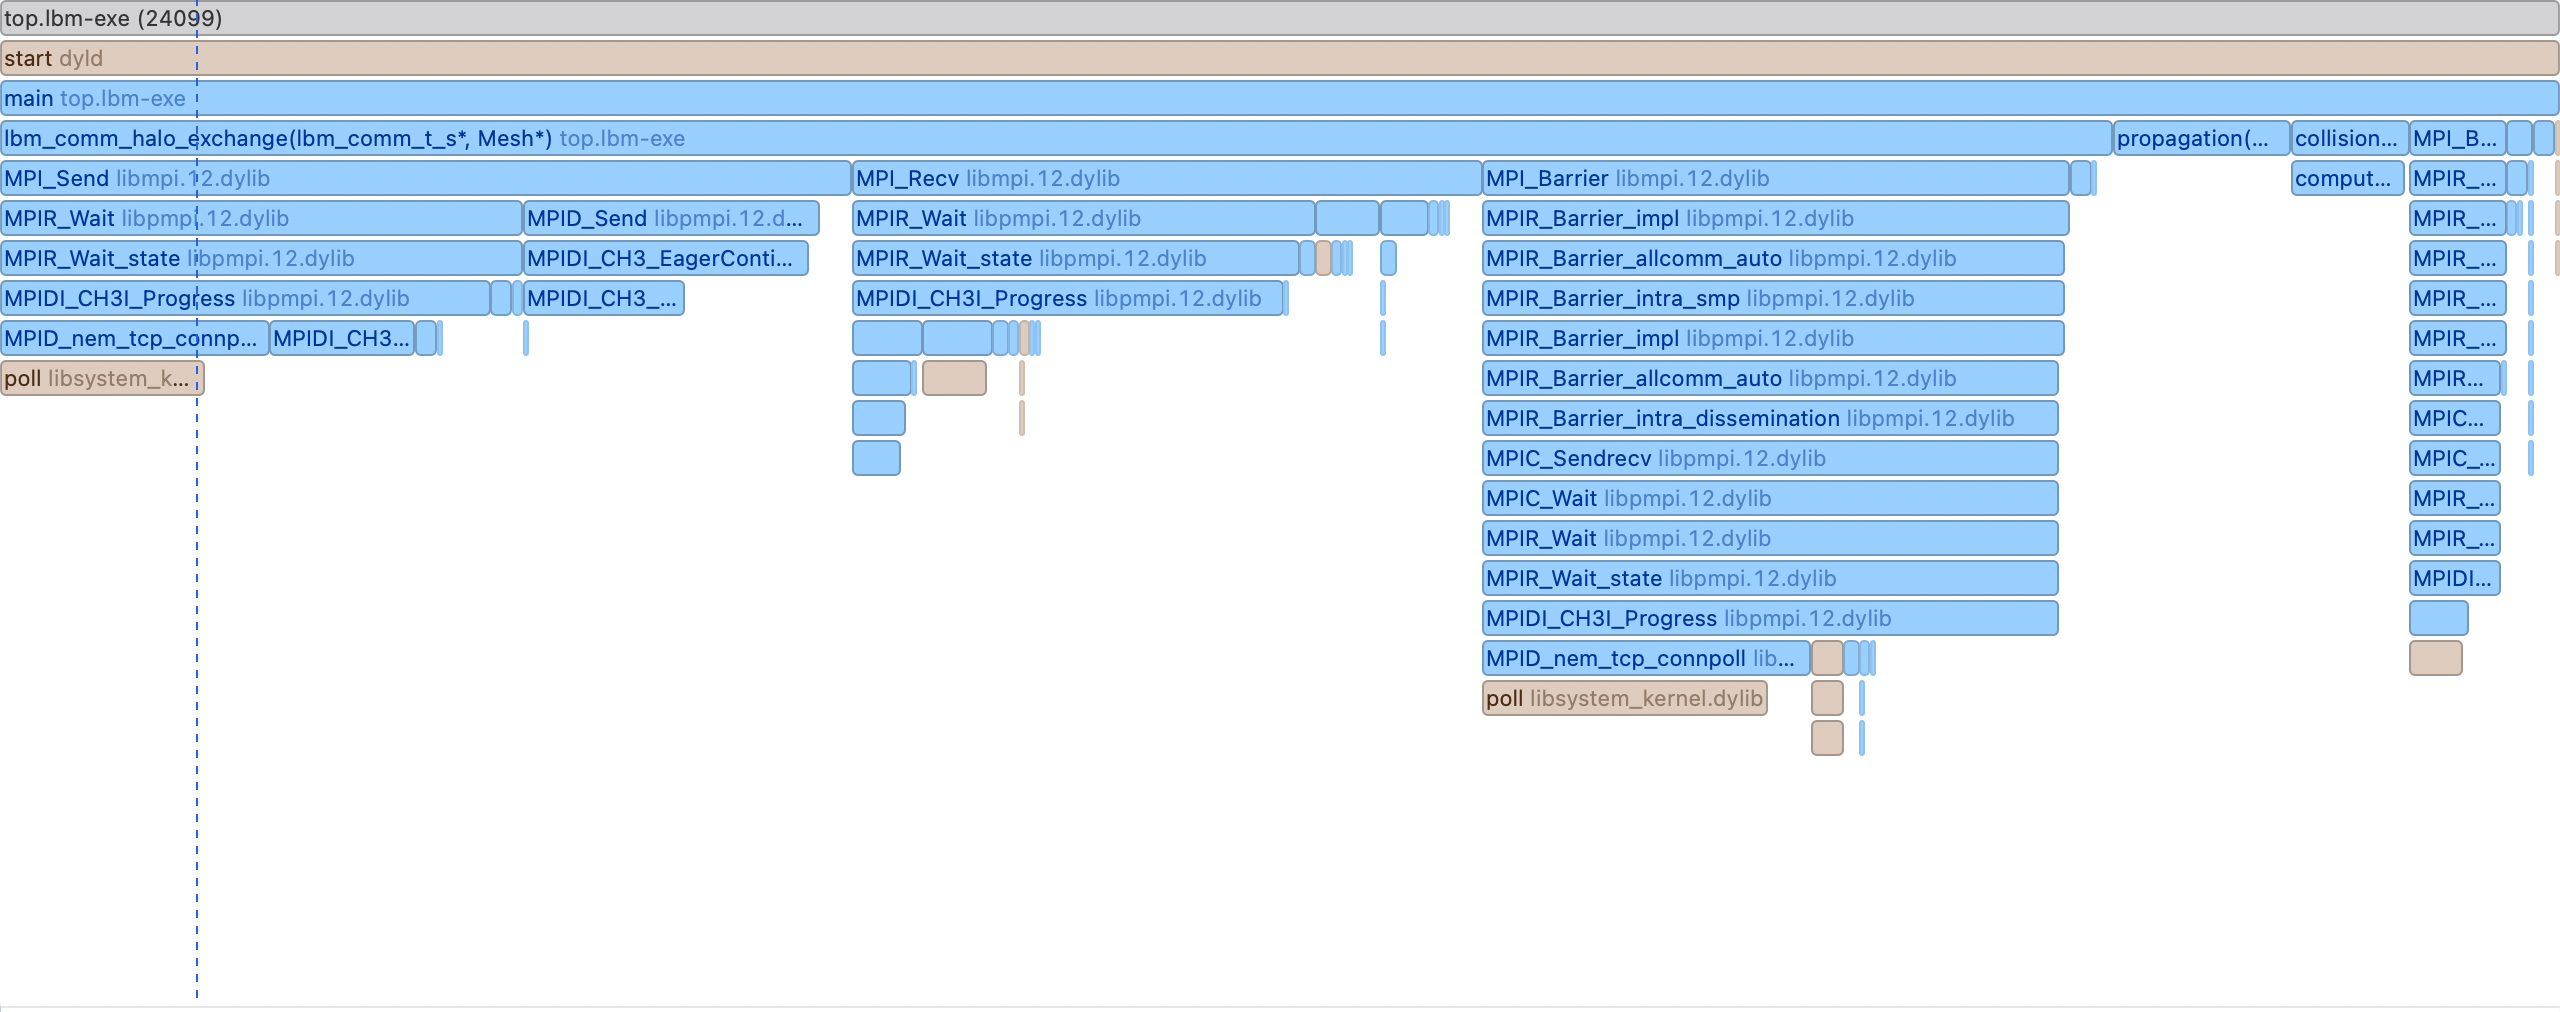
\includegraphics[scale=0.4]{graphs/flame graph 1.png}
  \label{fig:flamegraph1}
\end{figure}

\section{Fonction \textit{lbm\_comm\_halo\_exchange} initiale}
\label{section:AnnexeB}

\begin{lstlisting}[basicstyle=\tiny][language=Caml, caption=Python example]

void lbm_comm_halo_exchange(lbm_comm_t* mesh, Mesh* mesh_to_process) {
  int rank;
  MPI_Comm_rank(MPI_COMM_WORLD, &rank);

  lbm_comm_sync_ghosts_horizontal(mesh, mesh_to_process, COMM_SEND, mesh->right_id, mesh->width - 2);
  lbm_comm_sync_ghosts_horizontal(mesh, mesh_to_process, COMM_RECV, mesh->left_id, 0);
  MPI_Barrier(MPI_COMM_WORLD);

  lbm_comm_sync_ghosts_horizontal(mesh, mesh_to_process, COMM_SEND, mesh->left_id, 1);
  lbm_comm_sync_ghosts_horizontal(mesh, mesh_to_process, COMM_RECV, mesh->right_id, mesh->width - 1);
  MPI_Barrier(MPI_COMM_WORLD);

  lbm_comm_sync_ghosts_vertical(mesh_to_process, COMM_SEND, mesh->bottom_id, mesh->height - 2);
  lbm_comm_sync_ghosts_vertical(mesh_to_process, COMM_RECV, mesh->top_id, 0);
  MPI_Barrier(MPI_COMM_WORLD);

  lbm_comm_sync_ghosts_vertical(mesh_to_process, COMM_SEND, mesh->top_id, 1);
  lbm_comm_sync_ghosts_vertical(mesh_to_process, COMM_RECV, mesh->bottom_id, mesh->height - 1);
  MPI_Barrier(MPI_COMM_WORLD);

  lbm_comm_sync_ghosts_diagonal(mesh_to_process, COMM_SEND, mesh->corner_id[CORNER_TOP_LEFT], 1, 1);
  lbm_comm_sync_ghosts_diagonal(mesh_to_process, COMM_RECV, mesh->corner_id[CORNER_BOTTOM_RIGHT], mesh->width - 1,  mesh->height - 1);
  MPI_Barrier(MPI_COMM_WORLD);

  lbm_comm_sync_ghosts_diagonal(mesh_to_process, COMM_SEND, mesh->corner_id[CORNER_BOTTOM_LEFT], 1, mesh->height - 2);
  lbm_comm_sync_ghosts_diagonal(mesh_to_process, COMM_RECV, mesh->corner_id[CORNER_TOP_RIGHT], mesh->width - 1, 0);
  MPI_Barrier(MPI_COMM_WORLD);

  lbm_comm_sync_ghosts_diagonal(mesh_to_process, COMM_SEND, mesh->corner_id[CORNER_TOP_RIGHT], mesh->width - 2, 1);
  lbm_comm_sync_ghosts_diagonal(mesh_to_process, COMM_RECV, mesh->corner_id[CORNER_BOTTOM_LEFT], 0, mesh->height - 1);
  MPI_Barrier(MPI_COMM_WORLD);

  lbm_comm_sync_ghosts_diagonal(mesh_to_process, COMM_SEND, mesh->corner_id[CORNER_BOTTOM_LEFT], 1, mesh->height - 2);
  lbm_comm_sync_ghosts_diagonal(mesh_to_process, COMM_RECV, mesh->corner_id[CORNER_TOP_RIGHT], mesh->width - 1, 0);
  MPI_Barrier(MPI_COMM_WORLD);

  lbm_comm_sync_ghosts_diagonal(mesh_to_process, COMM_SEND, mesh->corner_id[CORNER_BOTTOM_RIGHT], mesh->width - 2, mesh->height - 2);
  lbm_comm_sync_ghosts_diagonal(mesh_to_process, COMM_RECV, mesh->corner_id[CORNER_TOP_LEFT], 0, 0);
  MPI_Barrier(MPI_COMM_WORLD);

  lbm_comm_sync_ghosts_horizontal(mesh, mesh_to_process, COMM_SEND, mesh->left_id, 1);
  lbm_comm_sync_ghosts_horizontal(mesh, mesh_to_process, COMM_RECV, mesh->right_id, mesh->width - 1);

  MPI_Syncall(MPI_COMM_WORLD);
}
\end{lstlisting}



\section{Flame Graph après optimisation MPI: Instruments.app}

\begin{figure}[H]
  \centering
  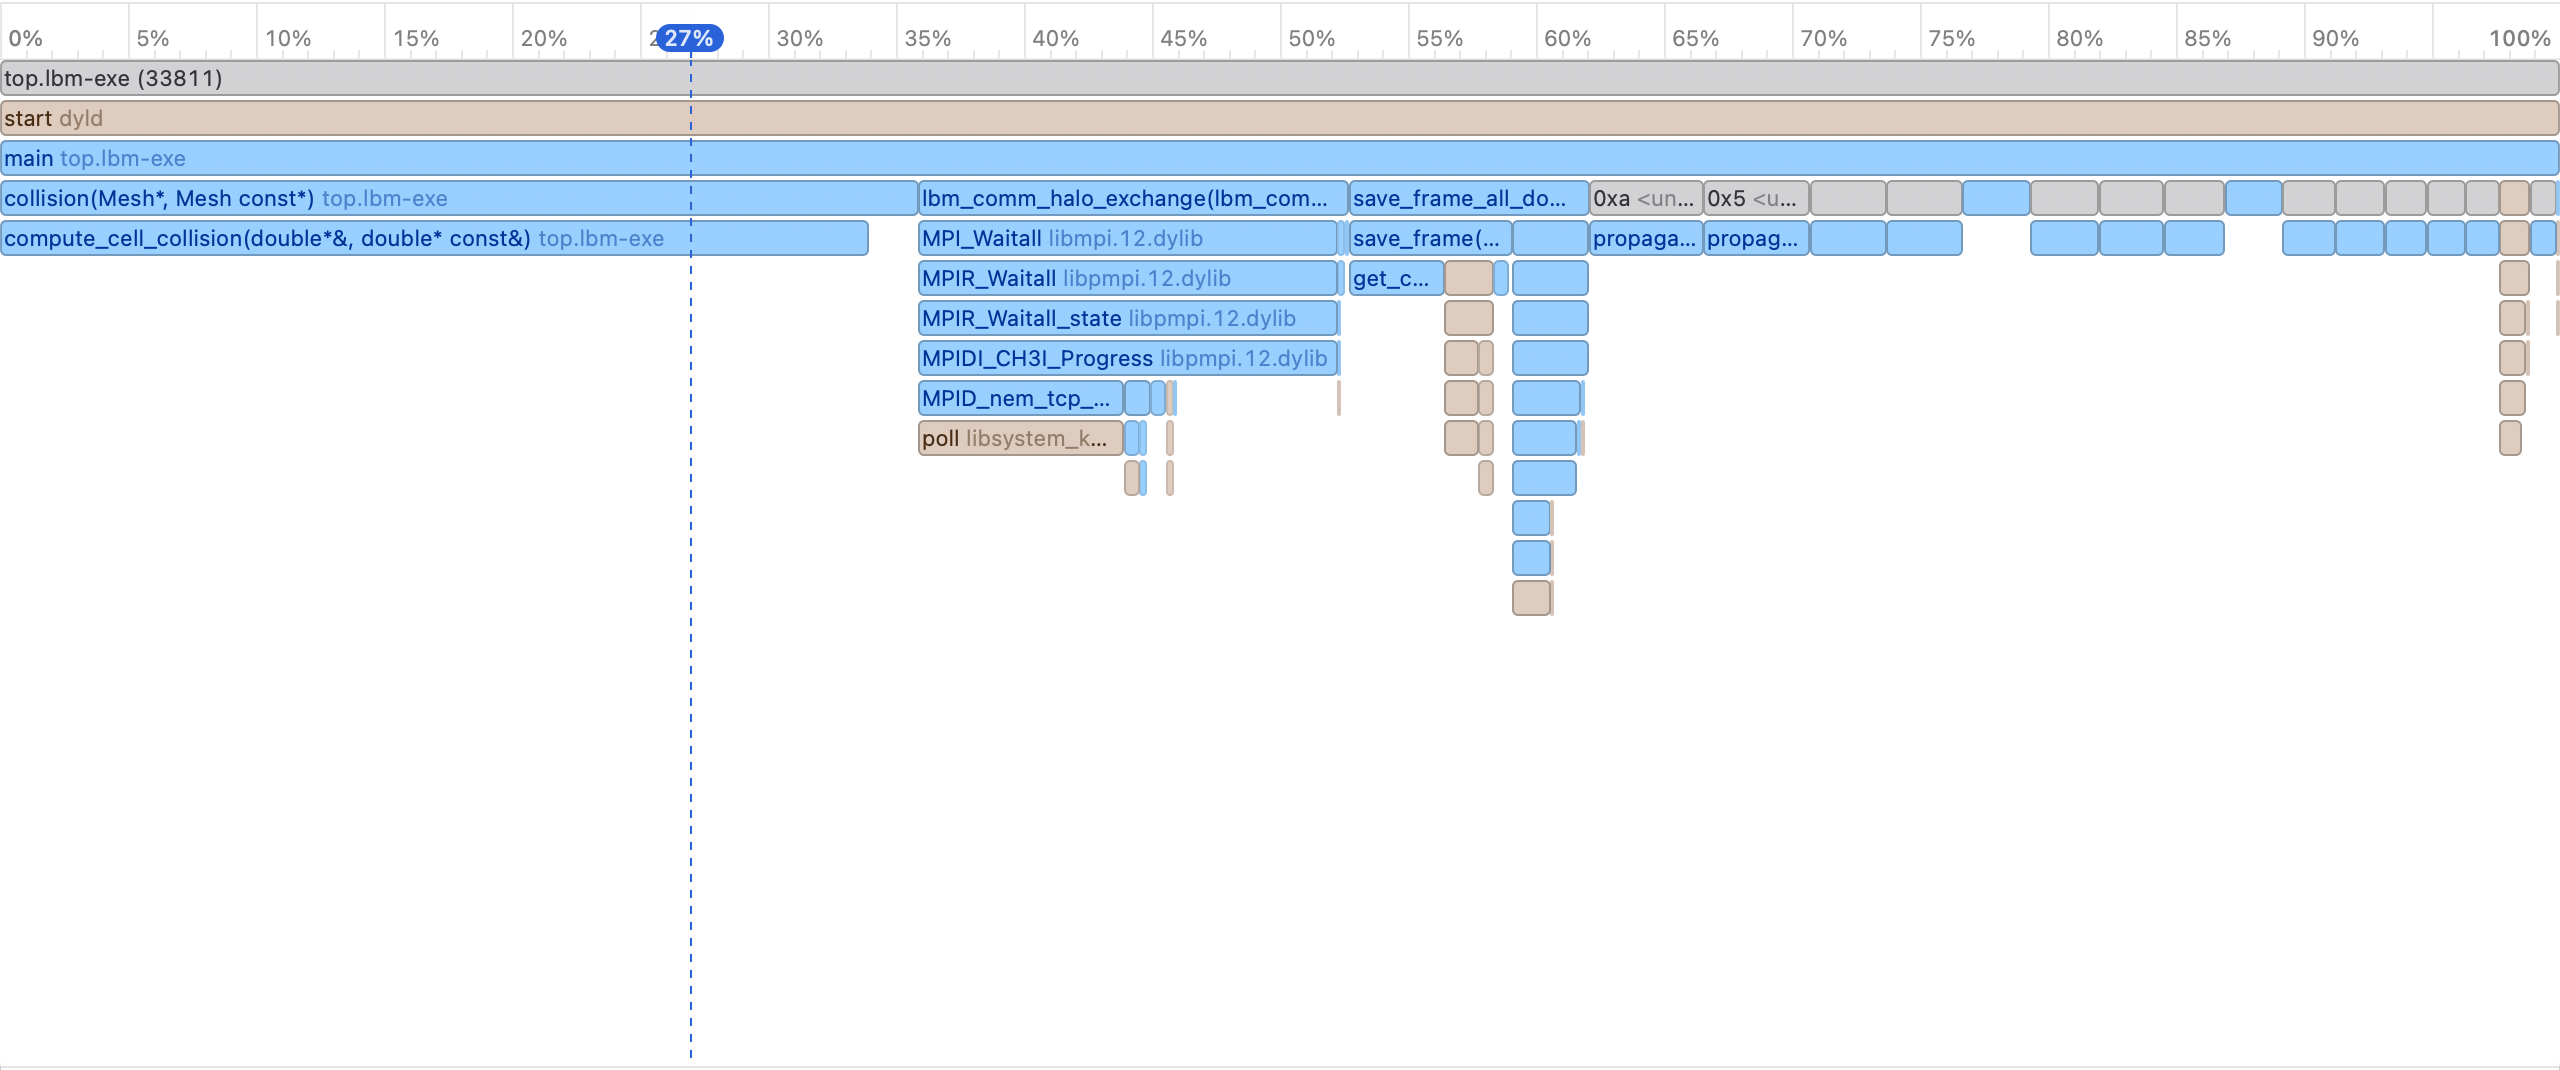
\includegraphics[scale=0.4]{graphs/flame graph 2.png}
  \label{fig:flamegraph2}
\end{figure}


\section{Comparaison version naïve et optimisée de cache-miss ratio}
\begin{figure}[H]
  \centering
  \begin{subfigure}{1.0\textwidth}
    \centering
    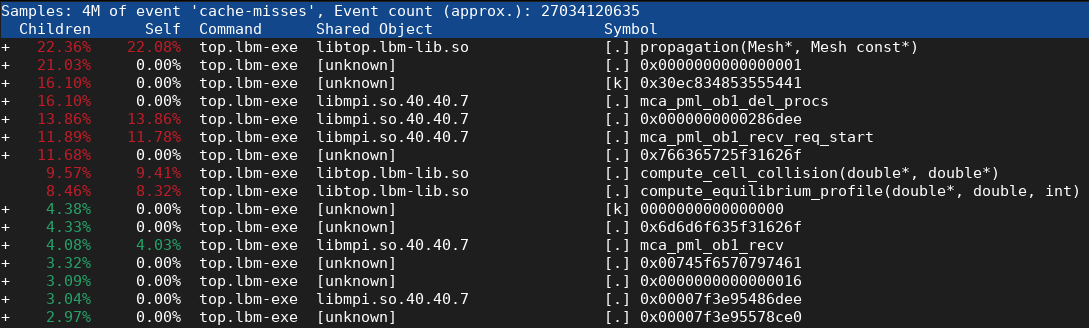
\includegraphics[scale=0.6]{graphs/miss-naive.png}
    \caption{Cache-misses version naïve}    
  \end{subfigure}
    \begin{subfigure}{1.0\textwidth}
    \centering
    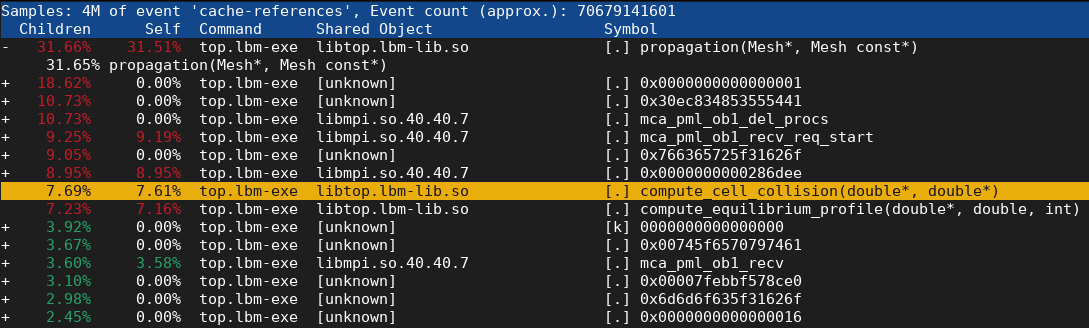
\includegraphics[scale=0.6]{graphs/ref-naive.png}
    \caption{Cache-references version naïve}
    \label{fig:perf-naive}
  \end{subfigure}
    \begin{subfigure}{1.0\textwidth}
    \centering
    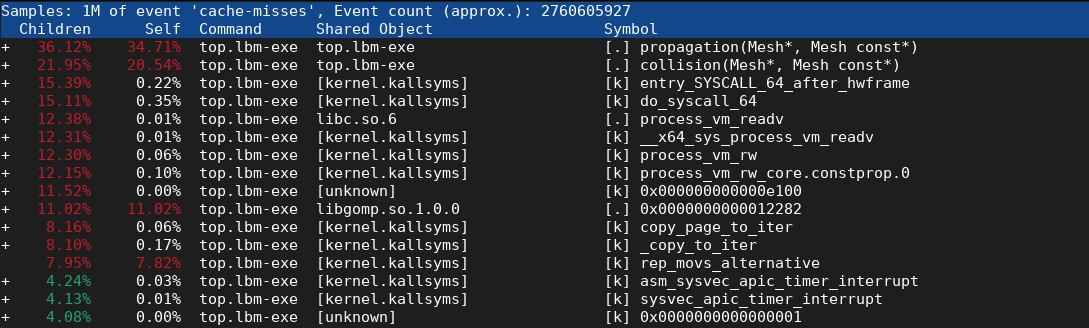
\includegraphics[scale=0.6]{graphs/miss-opti.png}
    \caption{cache-misses version optimisée}    
  \end{subfigure}
    \begin{subfigure}{1.0\textwidth}
    \centering
    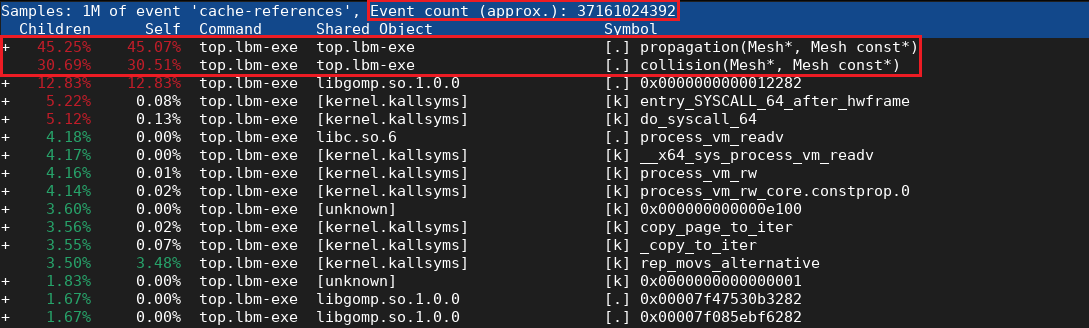
\includegraphics[scale=0.6]{graphs/ref-opti.png}
    \caption{cache-references version optimisée}
  \end{subfigure}
\end{figure}



\end{document}